\documentclass[11pt]{article}
\usepackage{graphicx}
\usepackage{enumitem}
\usepackage{lipsum}

%\usepackage{subfig}


%%%%%%%%%%%%%%%%%%%%%%%%%%%%%%%%%%%%%%%%%%%%%%%%%%%%%%%%%%%%%%%%%%%%%%%%%%%%%%%%
% packages
%%%%%%%%%%%%%%%%%%%%%%%%%%%%%%%%%%%%%%%%%%%%%%%%%%%%%%%%%%%%%%%%%%%%%%%%%%%%%%%%

\usepackage{coling2020}
\usepackage{times}
\usepackage{url}
\usepackage{amsmath,amsfonts}
\usepackage{latexsym}
\usepackage{hyperref}
\hypersetup{
  colorlinks   = true, %Colours links instead of ugly boxes
  urlcolor     = blue, %Colour for external hyperlinks
  linkcolor    = blue, %Colour of internal links
  citecolor    = blue  %Colour of citations
}
\usepackage{CJKutf8}
\usepackage{subfig}
\usepackage[sort&compress,round,comma,authoryear]{natbib}

%%%%%%%%%%%%%%%%%%%%%%%%%%%%%%%%%%%%%%%%%%%%%%%%%%%%%%%%%%%%%%%%%%%%%%%%%%%%%%%%
% latex functions
%%%%%%%%%%%%%%%%%%%%%%%%%%%%%%%%%%%%%%%%%%%%%%%%%%%%%%%%%%%%%%%%%%%%%%%%%%%%%%%%

\newcommand{\ltwo}[1]{\lVert{#1}\rVert}
\newcommand{\indicator}[1]{\mathbbm{1}\!\left[{#1}\right]}
\newcommand{\R}{\mathbb R}
\newcommand{\TEXT}{\texttt{text}}

\newcommand{\defn}[1]{\emph{{#1}}}
\newcommand{\fixme}[1]{{\color{red} \textbf{FIXME:} {\textit {#1}}}}
\newcommand{\XXX}{\textbf{XXX}~}
\newcommand{\bertmoji}{\texttt{BERTmoji}}
\newcommand{\bertmojill}{\texttt{BERTmoji-LL}}
\newcommand{\bert}{\texttt{BERT-multilingual}}

\DeclareMathOperator*{\argmax}{arg\,max}
\DeclareMathOperator*{\argmin}{arg\,min}
\DeclareMathOperator{\acc}{acc}
\DeclareMathOperator{\none}{\texttt{None}}
\DeclareMathOperator{\model}{\texttt{BERTMultilingualEmoticon}}
\DeclareMathOperator{\emoticon}{\texttt{TwitterEmoticon}}
\DeclareMathOperator{\emoticonTrain}{\texttt{TwitterEmoticon\_train}}
\DeclareMathOperator{\emoticonValid}{\texttt{TwitterEmoticon\_valid}}
\DeclareMathOperator{\emoticonTest}{\texttt{TwitterEmoticon\_test}}
\DeclareMathOperator{\corona}{\texttt{TwitterCorona}}

%%%%%%%%%%%%%%%%%%%%%%%%%%%%%%%%%%%%%%%%%%%%%%%%%%%%%%%%%%%%%%%%%%%%%%%%%%%%%%%%
% paper configuration
%%%%%%%%%%%%%%%%%%%%%%%%%%%%%%%%%%%%%%%%%%%%%%%%%%%%%%%%%%%%%%%%%%%%%%%%%%%%%%%%

%\setlength\titlebox{5cm}
%\colingfinalcopy % Uncomment this line for the final submission

% You can expand the titlebox if you need extra space
% to show all the authors. Please do not make the titlebox
% smaller than 5cm (the original size); we will check this
% in the camera-ready version and ask you to change it back.


\title{$\bertmoji$ says: "wear a mask" :  
\includegraphics[scale=0.07]{images/mask_photo.png}}

\author{First Author \\
  Affiliation / Address line 1 \\
  Affiliation / Address line 2 \\
  Affiliation / Address line 3 \\
  {\tt email@domain} \\\And
  Second Author \\
  Affiliation / Address line 1 \\
  Affiliation / Address line 2 \\
  Affiliation / Address line 3 \\
  {\tt email@domain} \\}

\date{}

%%%%%%%%%%%%%%%%%%%%%%%%%%%%%%%%%%%%%%%%%%%%%%%%%%%%%%%%%%%%%%%%%%%%%%%%%%%%%%%%
% document text
%%%%%%%%%%%%%%%%%%%%%%%%%%%%%%%%%%%%%%%%%%%%%%%%%%%%%%%%%%%%%%%%%%%%%%%%%%%%%%%%

\begin{document}
\maketitle
\begin{abstract}
    %There are no multi-lingual emoji prediction models. This makes it hard to investigate
    %how different languages use emojis. We present $\bertmoji$, a multi-lingual model 
    %that fine tunes the \texttt{BERTMultilingual} to the emoji prediction task.
    Emojis are a widely used tool for encoding emotional content in informal messages,
    and predicting which emoji corresponds to a piece of text can be used as a proxy for measuring the emotional content in the text.
    This paper presents the first model for predicting emojis in multilingual text.
    Our $\bertmoji$ model is a fine-tuned version of the $\bert$ model which supports 104 different languages.
    We trained our $\bertmoji$ model on \XXX million geolocated tweets sent in the first 6 months of 2020,
    and we apply the model to a case study analyzing coronavirus responses throughout the world. We were able to achieve an F1-score of 21 \% across the different languages and by applying this model to the coronavirus responses and mapping those emoji response to the Plutchik wheel; we tapped into the peoples' sentiment throughout the COVID-19 timeline. 
    \fixme{Add a 1 sentence summary of the results?}
\end{abstract}

%
% The following footnote without marker is needed for the camera-ready
% version of the paper.
% Comment out the instructions (first text) and uncomment the 8 lines
% under "final paper" for your variant of English.
% 
\blfootnote{
    %
    % for review submission
    %
    \hspace{-0.65cm}  % space normally used by the marker
    Place licence statement here for the camera-ready version. 
    %
    % % final paper: en-uk version 
    %
    % \hspace{-0.65cm}  % space normally used by the marker
    % This work is licensed under a Creative Commons 
    % Attribution 4.0 International Licence.
    % Licence details:
    % \url{http://creativecommons.org/licenses/by/4.0/}.
    % 
    % % final paper: en-us version 
    %
    % \hspace{-0.65cm}  % space normally used by the marker
    % This work is licensed under a Creative Commons 
    % Attribution 4.0 International License.
    % License details:
    % \url{http://creativecommons.org/licenses/by/4.0/}.
}





\section{Introduction}
\label{sec:intro}

Emoji Prediction is the task of identifying the correct emoji from natural language data such as Tweets. Such task has already been explored by \cite{Zhang2019}, where by adopting a transfer model based on the pre-trained BERT model \cite{devlin2018bert}, they achieved an F1-score of 38.52 \% on enlgish tweets. Previous work includes \cite{barbieri-etal-2018-semeval}, which offered 2 sub-tasks for multilingual emoji-prediction: English and Spanish. While the top team \cite{coltekin-etal-2018-tubingen} achieved F1-scores of 35.99\% and 22.36\% for the two respective tasks; by using an SVM classifier with bag-of-n-grams, we believe that the multilingual aspect of emoji prediction is not met when only serving 2 languages.


On the domain of Pre-trained models for Multi-lingual Natural Language Tasks, NVIDIA's researchers have published
\cite{puri2018large} where by using Recurrent Neural Networks on a 40 GB Amazon Review dataset demonstrate 
the scalability and transfer of the RNNs. By utilizing mixed precision arithmetic and 
a 32k batch size distributed on 128 GPUs, they trained a character-level 4096-dimension mLSTM.
Furthermore, \cite{kant2018practical} claim that large-scale unsupervised language modeling combined 
with finetuning, provides a solution to the Multi-Emotion sentiment classification (Plutchik),
including those with label class imbalance and domain-specific context. By training an attention-based
transformer network on a Amazon 40 GB dataset, it outperforms the mLSTM model, while fine-tuning significantly 
improves performance for both Transformers and mLSTM.

A question that arises is in which way can the emoji prediction task aid further research. \cite{cates2018} and \cite{avyaz2017}  show promising results that emoticons can be used to predict sentiment. Analysis from \cite{avyaz2017} shows that the utilization of Emoji characters results in higher sentiment scores while \cite{cates2018} highlights promising results when trying to make the connection between emoticons and the sentiment of YouTube comments.  

In the times that we are facing, exploring the public's sentiment offers useful insight into how people react to situations of stress, anxiety and uncertainty. A perfect source to explore this is through Twitter's API.\cite{subasish2020} draws from tweets related to Covid19 and India and by using public available sentiment analysis tools explores the public's sentiment on a two sentiment basis (negative and positive). 
    


{\color{blue} \lipsum[1-4] }

\subsection{Contributions}

\begin{enumerate}
    \item 
        We introduce the $\emoticon$ dataset for training emotion prediction models.
    \item
        We introduce the $\bertmoji$ model for emotion prediction that fine tunes the $\bert$ model \citep{devlin2018bert} to the emotion prediction task. 
        $\model$ is the first multilingual model for emotion prediction,
        and we provide an open source Python interface wrapped in an easy to use PyPi package.
    \item
        We analyze the performance of our model with respect to different languages and cultures to provide the first cross-cultural analysis of emotion prediction.
    \item 
        We introduce the $\corona$ dataset of all geotagged tweets about the coronavirus sent before July 2020.
        We apply our $\model$ model to this dataset,
        and map out the public's emotional response to the coronavirus.
\end{enumerate}

\begin{figure}
    \centering
    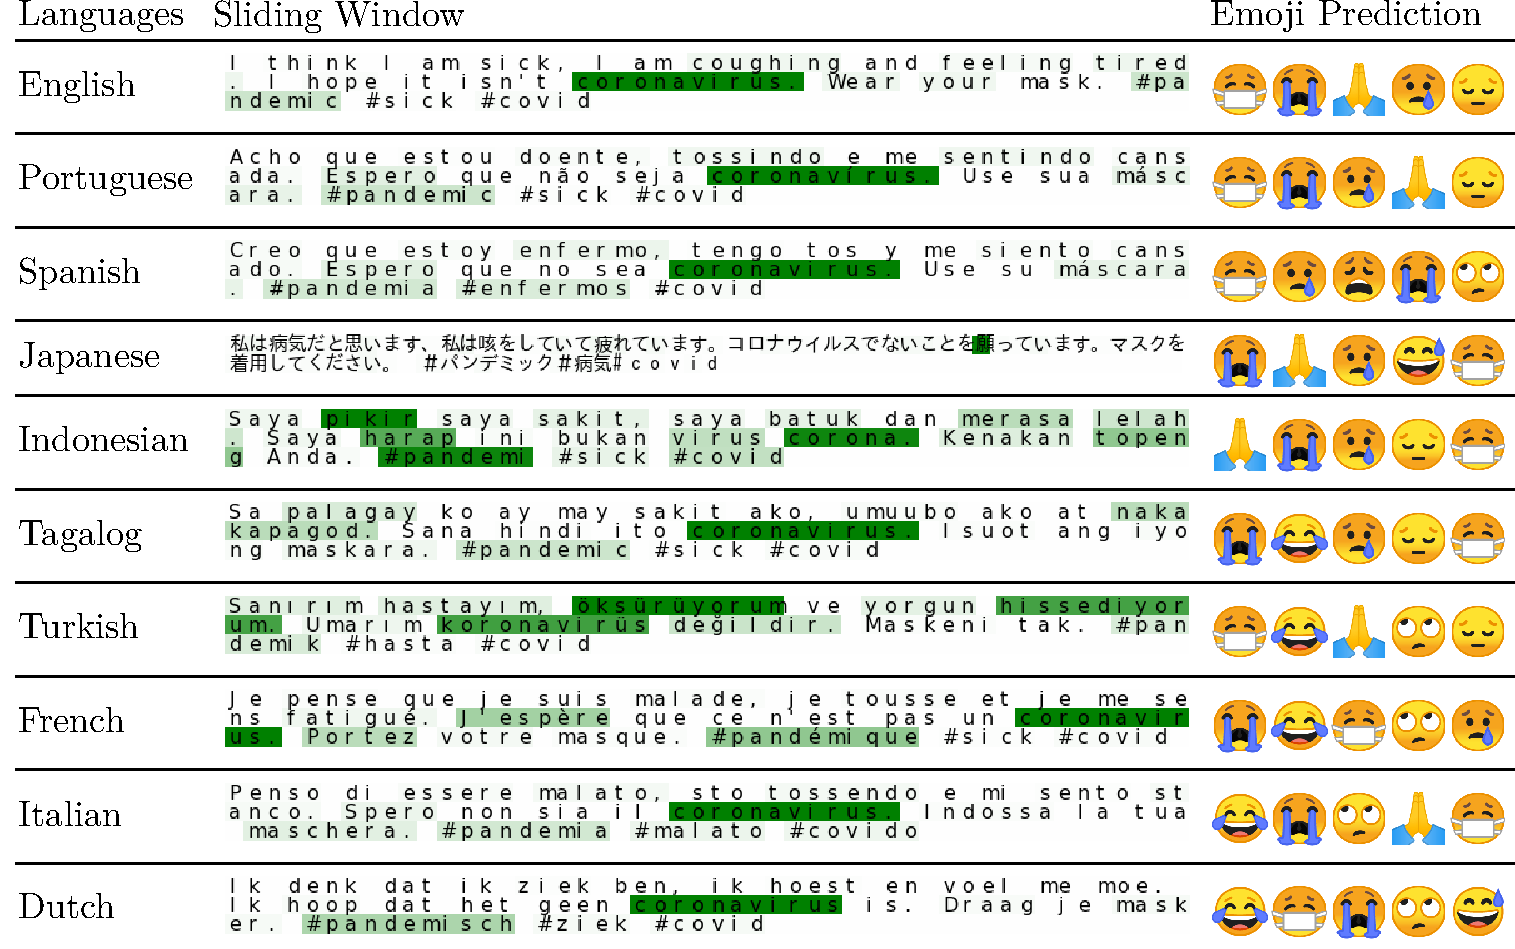
\includegraphics[width=\textwidth]{images/languages_slide_fix.pdf}
    \caption{
        $\bertmoji$ predicts good emojis in a wide variety of languages.
        All non-English text above was translated from the English using Google Translate.
        \fixme{The example tweet should be about coronavirus somehow. If you want the mask emoji in the title, then these should be predicting mask emojis here.}
        \fixme{Everything below Indonesian appears not to be working well; you should select an example where most of the languages work well.}
        \fixme{There's still a bit more that could be done to make the arabic and hindi text be rendered correctly.  The characters are all supposed to be connected, for example.  It would be okay if thi was done manually.  If you can't do this, then we might want to include Russian/Greek or something else that doesn't use latin characters.}
     }
    \label{fig:prediction_top10_langs}
\end{figure}

\subsection{Outline}

The remainder of our paper is structured as follows.

%%%%%%%%%%%%%%%%%%%%%%%%%%%%%%%%%%%%%%%%%%%%%%%%%%%%%%%%%%%%%%%%%%%%%%%%%%%%%%%%

\section{Training $\bertmoji$}

%%%%%%%%%%%%%%%%%%%%%%%%%%%%%%%%%%%%%%%%

\subsection{The $\emoticon$ Dataset}

The purpose of the $\emoticon$ dataset is to develop the emotion classifier which we will apply to the $\corona$ dataset.
The $\emoticon$ dataset is large, with \XXX million tweets in 66 languages sampled from the same distribution as our coronavirus tweets.
Therefore, we can expect a classifier trained on the $\emoticon$ dataset to transfer well to the $\corona$ dataset.

Following the work of \citet{fixme1,fixme2,fixme3}, we use emojis as distant labels for emotions.
Hand classifying text by emotions is an expensive and error prone process,
and the largest existing datasets for this task contain only about 10,000 tweets focusing on the limited domains of video games \citep{fixme} or stock performance \citep{fixme}.
The Unicode Standard \citep{fixme} currently defines over 3000 emojis,
most of which do not represent emotions.
In our analysis, we use only the original 80 emoji defined in the Unicode standard's emoticon code block (code points \texttt{0x1f600} - \texttt{0x1f650}).\footnote{
    In common usage, the words \defn{emoji} and \defn{emoticon} are interchangeable,
    but in this paper we adopt the Unicode Standard's definitions of these terms.
    By these definitions, an \defn{emoji} is any one of 3304 pictographs that are not part of any written language,
    and an \defn{emoticon} is one of the original 80 emoji.
}
We limit are analysis to emoticons only because:
they are the most commonly used emoji on twitter\footnote{
    See \url{http://www.emojitracker.com/} for real-time stats on Twitter emoji usage.
}
and each of these emoticons represents an emotion (emoticon is a portmanteau of emotion and icon).

To generate the $\emoticon$ dataset, 
we filtered the full set of geolocated tweets so that only tweets containing one of the 80 emoticons were included,
and any duplicate tweets were removed.
Then we preprocessed each tweet by replacing all user mentions with a special token \texttt{<mention>} and all URLs with a special token \texttt{<url>} and deleting all emojis.
We decided to keep all hashtags because hashtags can contain potentially valuable emotional content.
There exist a lot of tweets that contain multiple repetitions of emojis.
We address the issue similarly to how \cite{100_million_tweets} did where for each unique emoji we have a separate tweet with that emoji as a label. 
For tweets containing repetitions of the same emoji; we only save one instance of it.
Finally, each tweet is labelled with the emojis that were deleted from the tweet.
In total, the $\emoticon$ dataset contains 64.2 million tweets sent by 4.2 million users,
and the tweets are written in 66 different languages and were sent from 246 different countries.
Table \ref{table:lang} shows the total number of tweets per language,
and Figure \ref{fig:emoticons} shows the full list of emoticons and their counts in our dataset. 

\begin{figure}
    \centering
    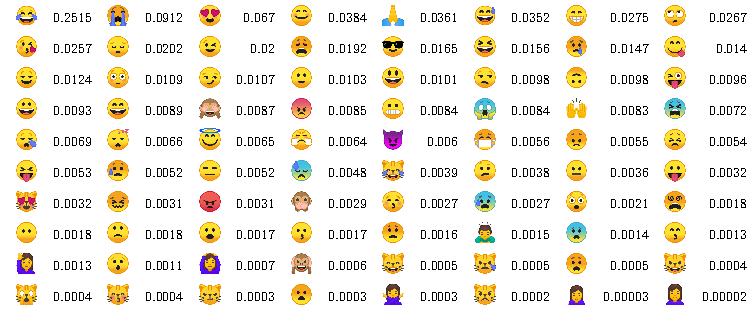
\includegraphics[scale = 1.2]{images/emojitable.pdf}
    \caption{The emoji distribution of the $\emoticon$ dataset.} 
    \label{table:lang}
\end{figure}

Our goal with this dataset is to construct a classifier that takes as input a tweet and outputs an emoticon that represents the emotion of the tweet.
In order to train this model properly,
we carefully split the $\emoticon$ dataset into training, validation, and test sets ensuring that no user is present in all three sets in order to prevent data leakage.
In particular we assign 80\% of users to the training set, 10\% to the validation set, and 10\% to the test set.
The tweets contained in each set are then the tweets sent by each of the users in the set.

Importantly, duplicate tweets are included in the $\corona$ dataset,
but they are not included in the $\emoticon$ dataset.
This is because of the purpose of the $\emoticon$ dataset. 
We aimed to apply our $\model$ to this dataset,
which is something with free user input where our training data is not fully representative of the eventual data our model will be applied to.
Therefore this limits our abilities to make assumptions and could possibly inflate our sense of model efficacy.
On the other hand when dealing with the $\corona$ dataset,
duplicate inputs result in some distribution on our outputs.
Since we want to map out the public's emotional response to the coronavirus, it is important 
for those distributions to be maintained.

%%%%%%%%%%%%%%%%%%%%%%%%%%%%%%%%%%%%%%%%

\subsection{Training Protocol}

To generate $\model$, we utilized the pre-trained BERT model \cite{bert} by fine-tuning it to our multilingual emoji prediction task. 
BERT is a new language representation model, which is aimed in pretraining deep bidirectional representations from unlabeled text by jointly conditioning on both left and right context in all layers.
Therefore, the pre-trained model can be easily fine-tuned by adding another output layer.
One of the reasons why we picked BERT is due to its performance on the General Language Understanding Evaluation (GLUE) \cite{} benchmark.
It is comprised of nine language understanding tasks, assembled from a diverse dataset which includes insight into model performance with respect to a wide range of linguistic phenomena.
At the time of writing, BERT and its variations hold a number of top achieving scores in the GLUE leader-board \ref{leaderboard}.   

\begin{figure}
    \centering
    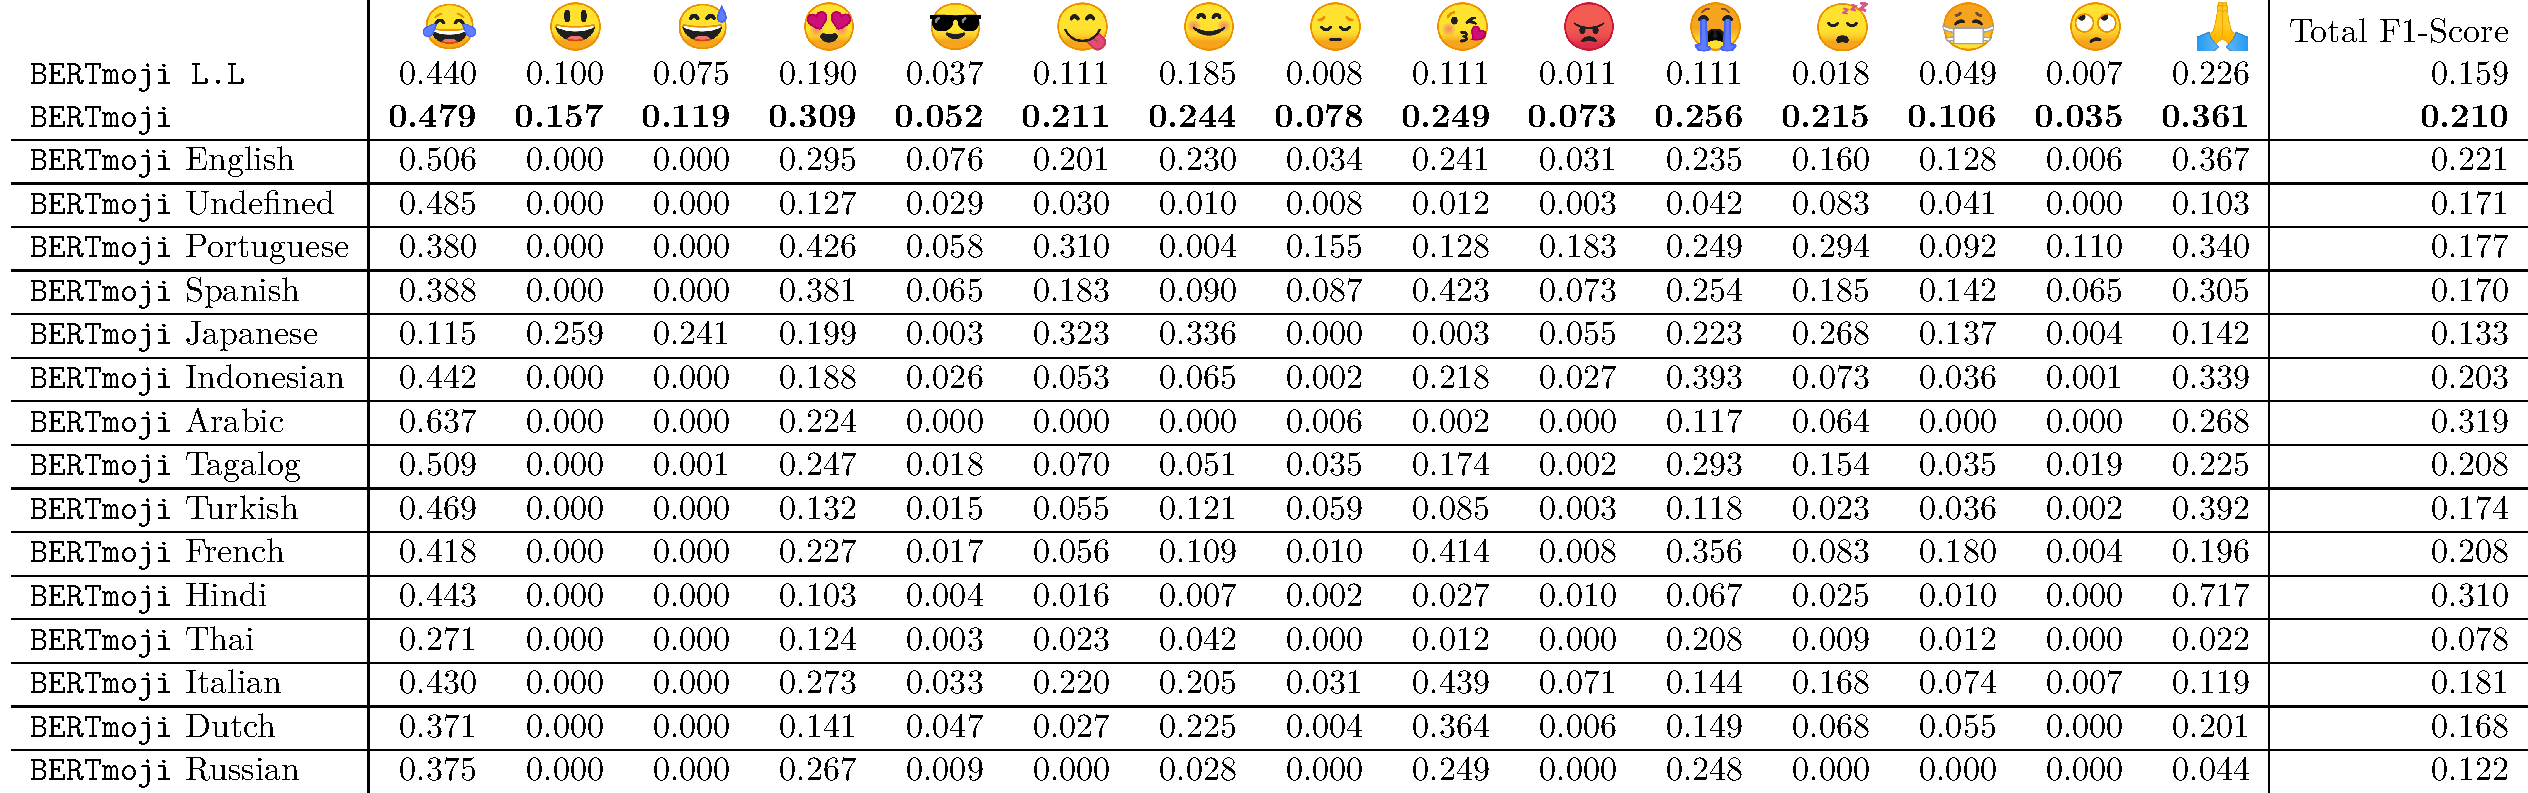
\includegraphics[width=\textwidth]{images/f1_score_table_fix.pdf}
    \caption{
        F1 scores of the $\bertmojill$ and $\bertmoji$ model on 15 selected emojis. Included also are the F1-score language breakdown. (The total is this the sum of averages, kind of showing how we go an f1 score of 21\%).
        %$\bertmojill$ is the model where the last layer is trained. $\bertmoji$ is the fully trained model.
        \fixme{numbers should be right aligned, text should be left aligned}
        \fixme{The typography of the bert models needs to match the typography used in the rest of the paper.}
        \fixme{I don't understand what total/ave is.}
        \fixme{In the table, it needs to be absolutely clear that the languages are also $\bertmoji$.}
        \fixme{There's some really weird results here, like in the second and third columns, only Japanese does well on these emojis.  Why?  Do these emojis  occur more often in Japanese?}
    }
    \label{fig:tweets_per_day}
\end{figure}

For our model, we utilized the pre-trained "bert-base-multilingual-uncased" which includes 102 languages and it is comprised of: 12-layer, 768-hidden, 12-head and 110M parameters.
Therefore, we utilized the corresponding BERT tokenizer to encode our data.
We fine-tuned this pre-trained model to generate two models. 
The first one only trained the last layer of the model, while the second one trained all the layers.
We followed the Train-Validation-Test split procedure, where 1 epoch took approximately 6 days to run on one Nvidia GeForce RTX 2080 graphics card.
The hyper-parameters with which we achieved the highest accuracies are the following. 
When training the last layer of the model we used: a learning-rate of 1e-04, Adam optimizer and gradient clipping. 
While training all the layers of the model we had: a learning-rate of 1e-05, Adam optimizer and gradient clipping. 
Both models were warm-started from previous runs and the batch size used was 64.

We now present the results of the models. We used the scikit-learn \cite{} library, to classify our models.
We executed 2 classification for the two models. Initially we measured the f1-scores for all 80 emoji categories.
The last-layer model had an F1-score of 15.89\% while the other one achieved an F1-score of 20.97\%. 
Afterwards, we performed the classification on the top-15, F1-score achieving emojis. 
Those emojis comprised about 70 percent of the dataset.
The results were the F1-scores of 24.07\% and 31.77\% accordingly.
All the F1-scores are calculated via weighted average. Figure 3,4 presents more detailed analysis of the results.
While f1-scores vary for different emojis and languages,
both figures highlight that  $\bertmoji$ outperforms $\bertmojill$. 

We now precede in testing $\bertmoji$ ability to predict emojis for different languages.
We decided on picking an English sentence that expressed emotions and could possibly appear in twitter,
we then translated from English to the other nine languages from Figure 2 using Google Translate.
The sentence was: "Thinking about all the things I didn't do today, ok bed time ... \#tired \#sleep."
In addition, we also applied the sliding window algorithm to the translated sentences,
in order to observe which words were more significant for the $\bertmoji$ across the translations.
The results are shown in Figure 6. 

\begin{figure}
    \centering
    \subfloat{{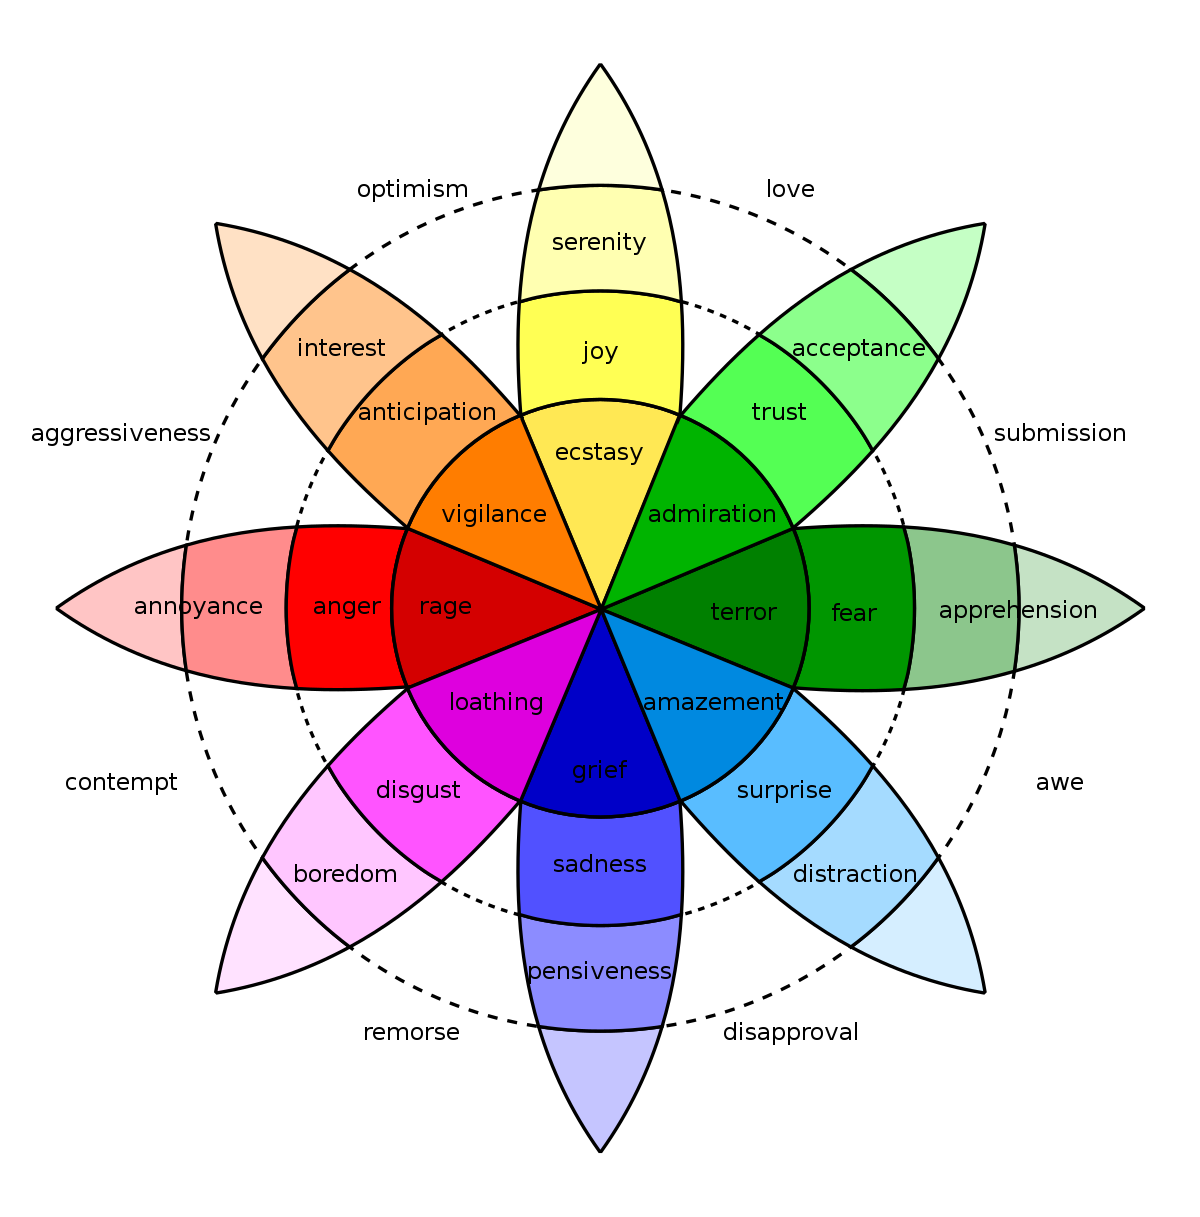
\includegraphics[scale=0.14]{images/Plutchik-wheel.png}}}%
    \label{fig:plu_wheel}
    \subfloat{{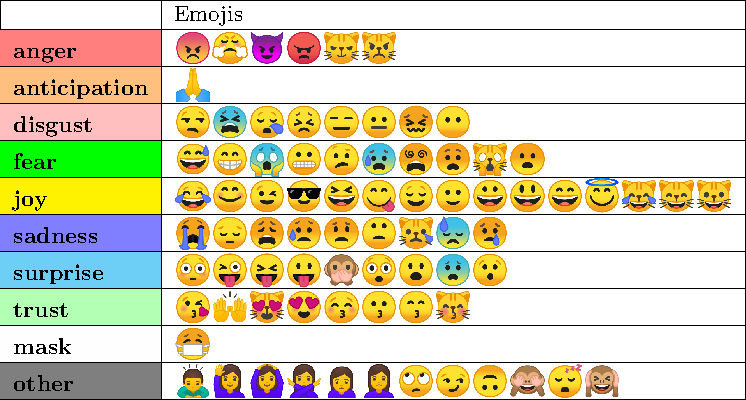
\includegraphics[scale= 0.79]{images/emoji_categories_fix.pdf}}}%
    \caption{
        (\emph{Left}) 
        The Plutchik wheel of emotions.
        %\footnote{\url{https://en.wikipedia.org/wiki/Robert_Plutchik}}
        (\emph{Right}) 
        We have grouped emojis into 10 different categories:
        8 emotional categories from the Plutchnik wheel,
        1 category for the ``face with medical mask'' emoji,
        and 1 category for all other emojis that do not clearly represent an emotion.
        \fixme{
            Text in tables is always left aligned.
        }
        \fixme{
            You need the horizontal bar at the top.
        }
        \fixme{
            Change ``mask emoji'' to just ``mask''
        }
        \fixme{
            Change the order of the rows so that the emotions are alphabetical.
        }
        \fixme{
            I'm still not 100\% satisfied with this breakdown of emojis into categories.
            I think there's a strong chance that a reviewer will find one emoji they don't think belongs into a category (especially with anticipation) and therefore discount all your results.
            If you have time to rerun experiments,
            I would make the anticipation category contain only the praying hands emoji,
            and move the remainder into either into the other category or other emotions
        }
    }
    \label{fig:Mapped_emojis}%
\end{figure}

%%%%%%%%%%%%%%%%%%%%%%%%%%%%%%%%%%%%%%%%

\subsection{Model Evaluation}

%%%%%%%%%%%%%%%%%%%%%%%%%%%%%%%%%%%%%%%%%%%%%%%%%%%%%%%%%%%%%%%%%%%%%%%%%%%%%%%%

\section{Coronavirus Case Study}

\subsection{The $\corona$ Dataset}

This section describes our two new Twitter datasets, $\corona$ and $\emoticon$.
To generate both datasets,
we first downloaded all geolocated\footnote{%
Twitter users can adjust their privacy settings to include different amounts of geolocation metadata.
In particular, they can include the exact GPS coordinate that a tweet was sent from,
an approximate location (for example, the city that the tweet was sent from),
or no location information at all.
We say that a tweet is \defn{geolocated} if any of this metadata is included about the tweet.
Approximate 1\% of all tweets are geolocated.
} 
tweets sent over the six month period from January 1st to June 30th, 2020.
This full dataset contains \XXX million tweets sent from \XXX users and from \XXX different countries.
The $\corona$ and $\emoticon$ datasets were then constructed by filtering this full dataset in different ways.

The goal of the $\corona$ dataset is to include any geolocated tweet that references the coronavirus in any language.
We use a relatively complicated process to extract these tweets in order to ensure maximum recall and precision in a wide range of languages.
Our procedure is:
\begin{enumerate}
\item
We generated a list of \XXX English-language search terms related to the coronavirus,
such as \texttt{coronavirus}, \texttt{covid19}, \texttt{wuhan} and \texttt{lockdown}.
We then used Bing's translation API to translate each of these terms into the 72 languages supported by Bing translate.
Table \ref{table:search_terms} in the supplemental material contains the full list of search terms in English and selected translations.
\item
We used Python's \texttt{spacy} library \citep{spacy2} to tokenize and lemmatize each of the \XXX million tweets in the full dataset.
\texttt{spacy} supports this process in 58 different languages,
and for each tweet we used the appropriate \texttt{spacy} module for the language specified in the tweet's metadata.
\item
Finally, the $\corona$ dataset is constructed as the set of all tweets whose lemmatized text contains any of the search terms from the tweet's language or English.
We include both languages in this filtering step because it is common for non-English tweets to use English words like \texttt{coronavirus} when referencing the virus.
\end{enumerate}
Table \ref{table:lang} shows the 54 languages that are supported by all 3 services along with the total number of tweets in each language.
Figure \ref{fig:tweets_per_day_sent} provides a summary of the number of tweets per day and Figure \ref{fig:corona:spatial} shows the spatial distribution of the tweets.

\begin{figure}%
    \centering
    \subfloat{{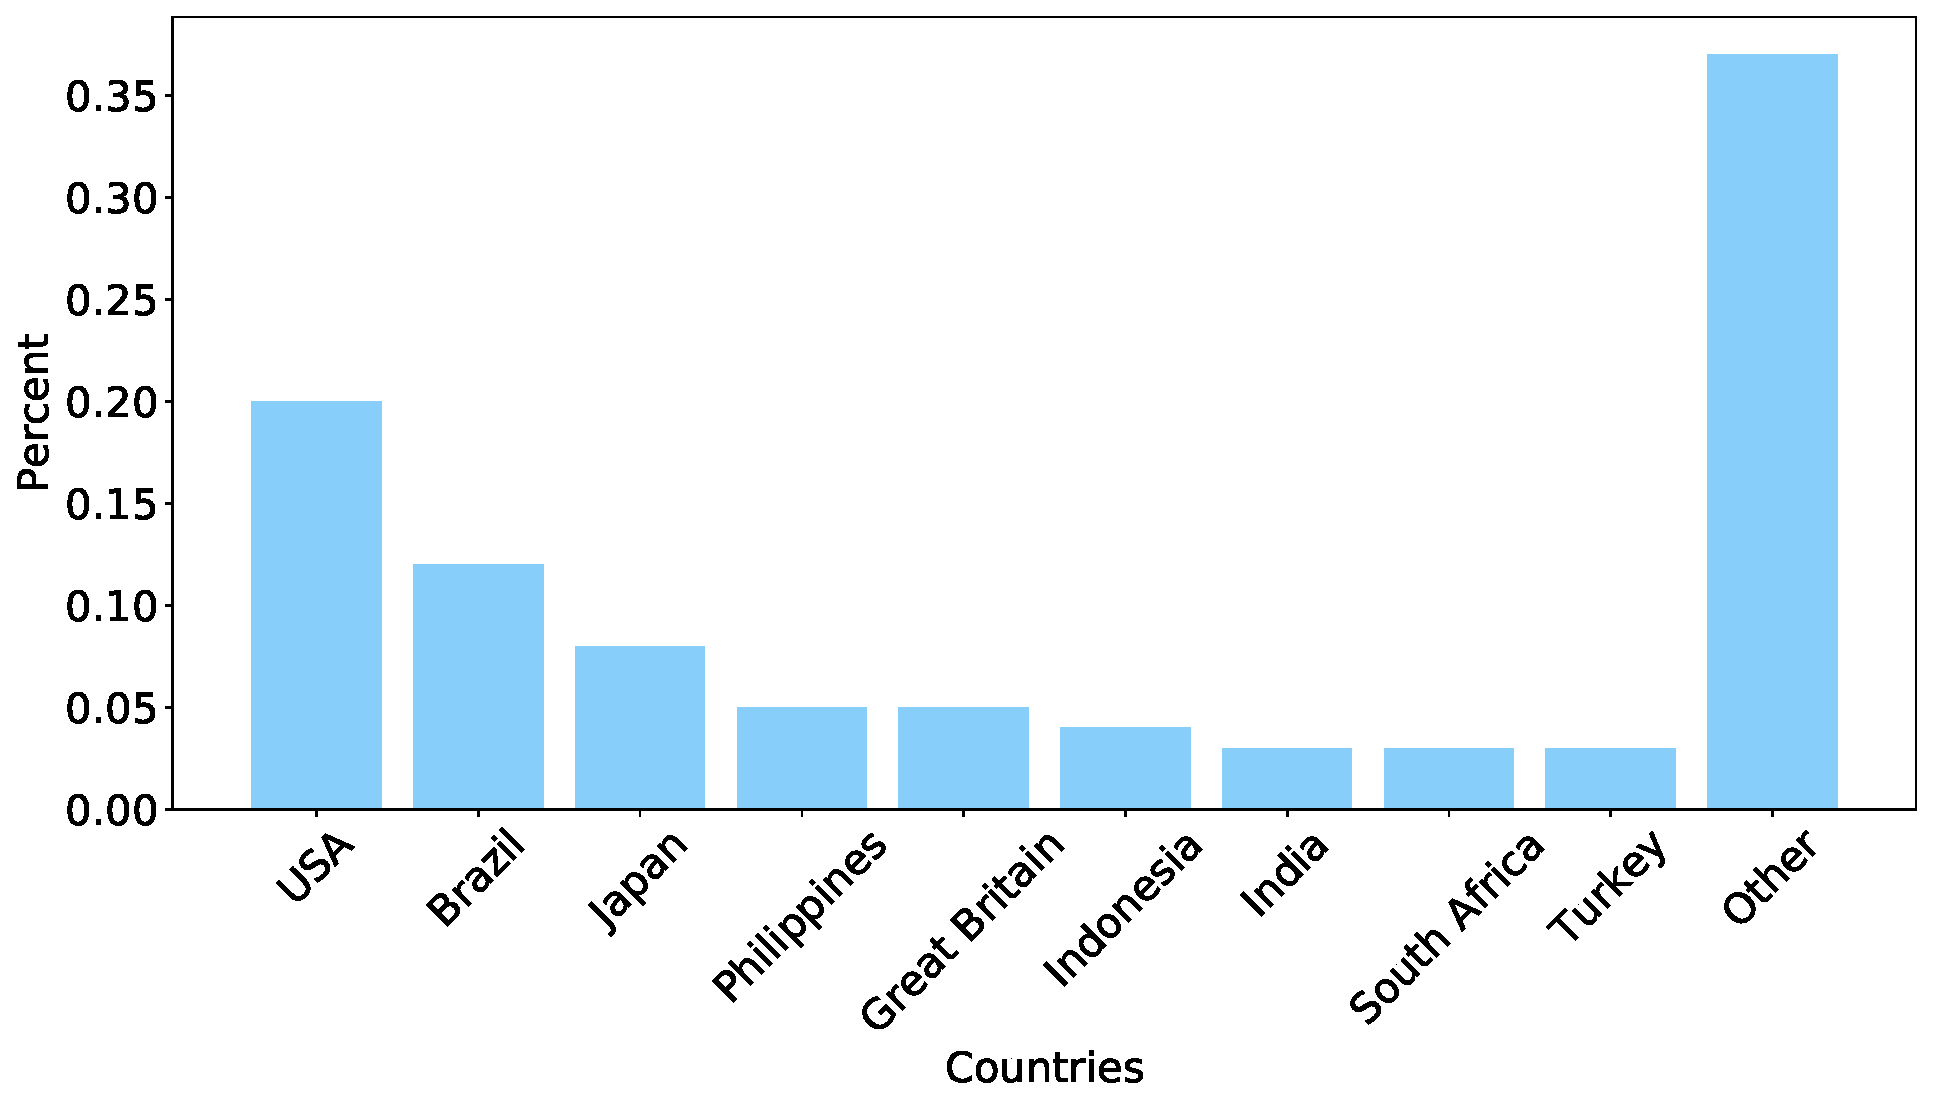
\includegraphics[scale=0.24]{images/dis_country.eps}}}%
    \label{adsad}
    \subfloat{{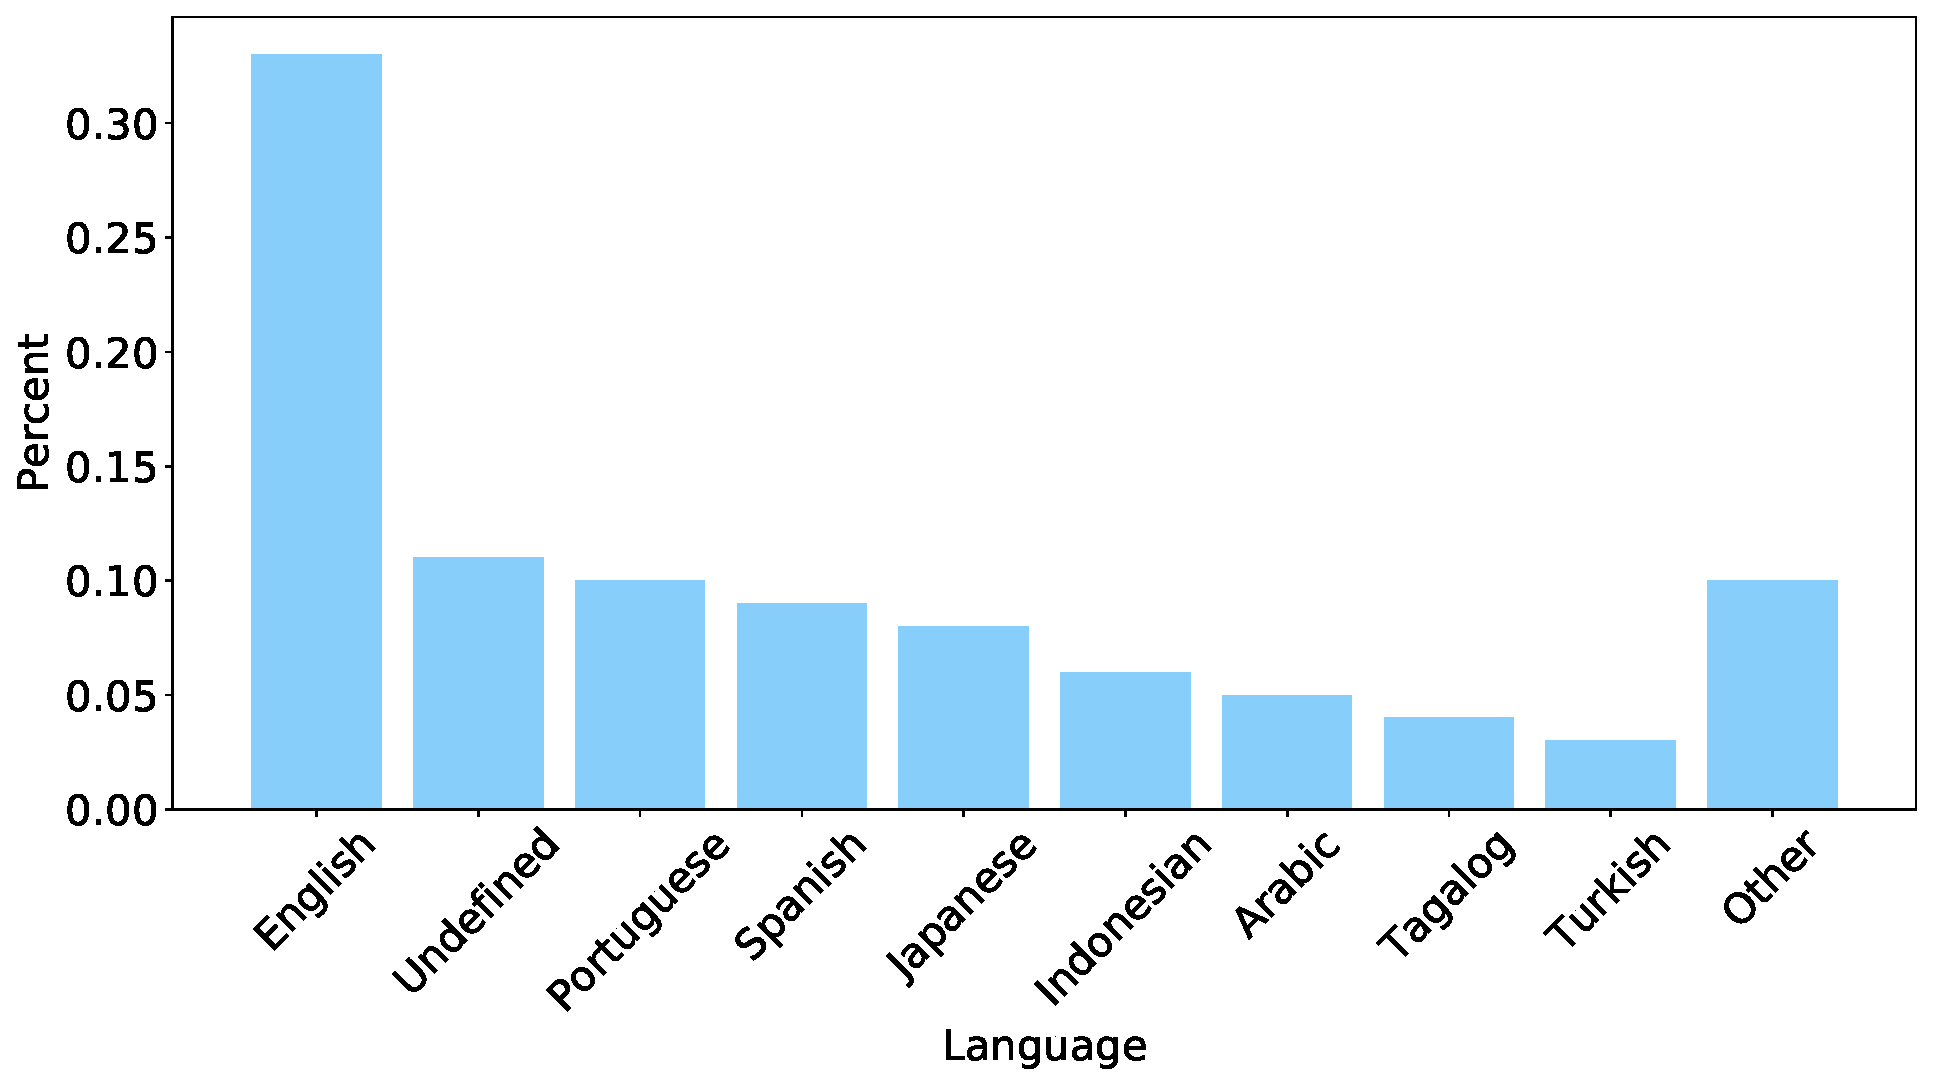
\includegraphics[scale =0.24]{images/dis_lang.eps} }}%
    \caption{ (\emph{Left}) The spatial distribution of the $\emoticon$ dataset. (\emph{Right}) The language distribution of the $\emoticon$ dataset.  }%
    \label{fig:example}%
\end{figure}


The other significant dataset of coronavirus related tweets is due to \citet{chen2020tracking}.
There are two main differences between our dataset and theirs.
First, we only include geolocated tweets,
whereas they include non-geolocated tweets as well.
This results in their dataset being about 50x larger than ours,
with about 250 million tweets over the same time period.
Because their data is not geolocated, however, their data is not suitable for the cultural analysis we perform in Section \ref{sec:}.
The second difference is that our dataset uses a more advanced language-aware filtering method.
They only search for tweets that contain English keywords.
Most languages, however, have few words in common with English,
and non-Latin based languages frequently do not even use the word \texttt{coronavirus} to describe the virus.
Chinese tweets, for example, commonly refer to the coronavirus with the string
\begin{CJK}{UTF8}{gbsn}
病毒
\end{CJK},
and Chinese-language tweets containing this string will get included in our dataset but not in their dataset.
As a result of this more advanced processing, the fraction of non-English tweets is much larger in our dataset than theirs (\XXX versus 38\%).
Again, this improves our multicultural analysis in Section \ref{sec:}.

We used NVidia's \texttt{sentiment-discovery} library to provide a preliminary sentiment analysis of the $\corona$ dataset,
and the results are shown in Figure \ref{fig:nvidia-sentiment}.
The results are not very informative, however, because NVidia's model was trained on a small set of English-language tweets (about 16 thousand) about video games,
and there is little reason to believe that this domain would transfer well to the coronavirus domain.

%%%%%%%%%%%%%%%%%%%%%%%%%%%%%%%%%%%%%%%%

\subsection{Results}

In the following section we explore one of the potential applications of the $\bertmoji$.
Since the Covid-19 outbreak, Twitter has become more than ever the place for participating in public discord, 
sharing opinions, and expressing thoughts. All of the preceding, are always charged with some type of sentiment.
While there exist a plethora of models that engage in sentiment analysis, the barrier of language prevents a lot 
of twitter data from being used,trained and analyzed. We however are able to circumvent that obstacle with the use of emojis.


\begin{figure}
    \centering
    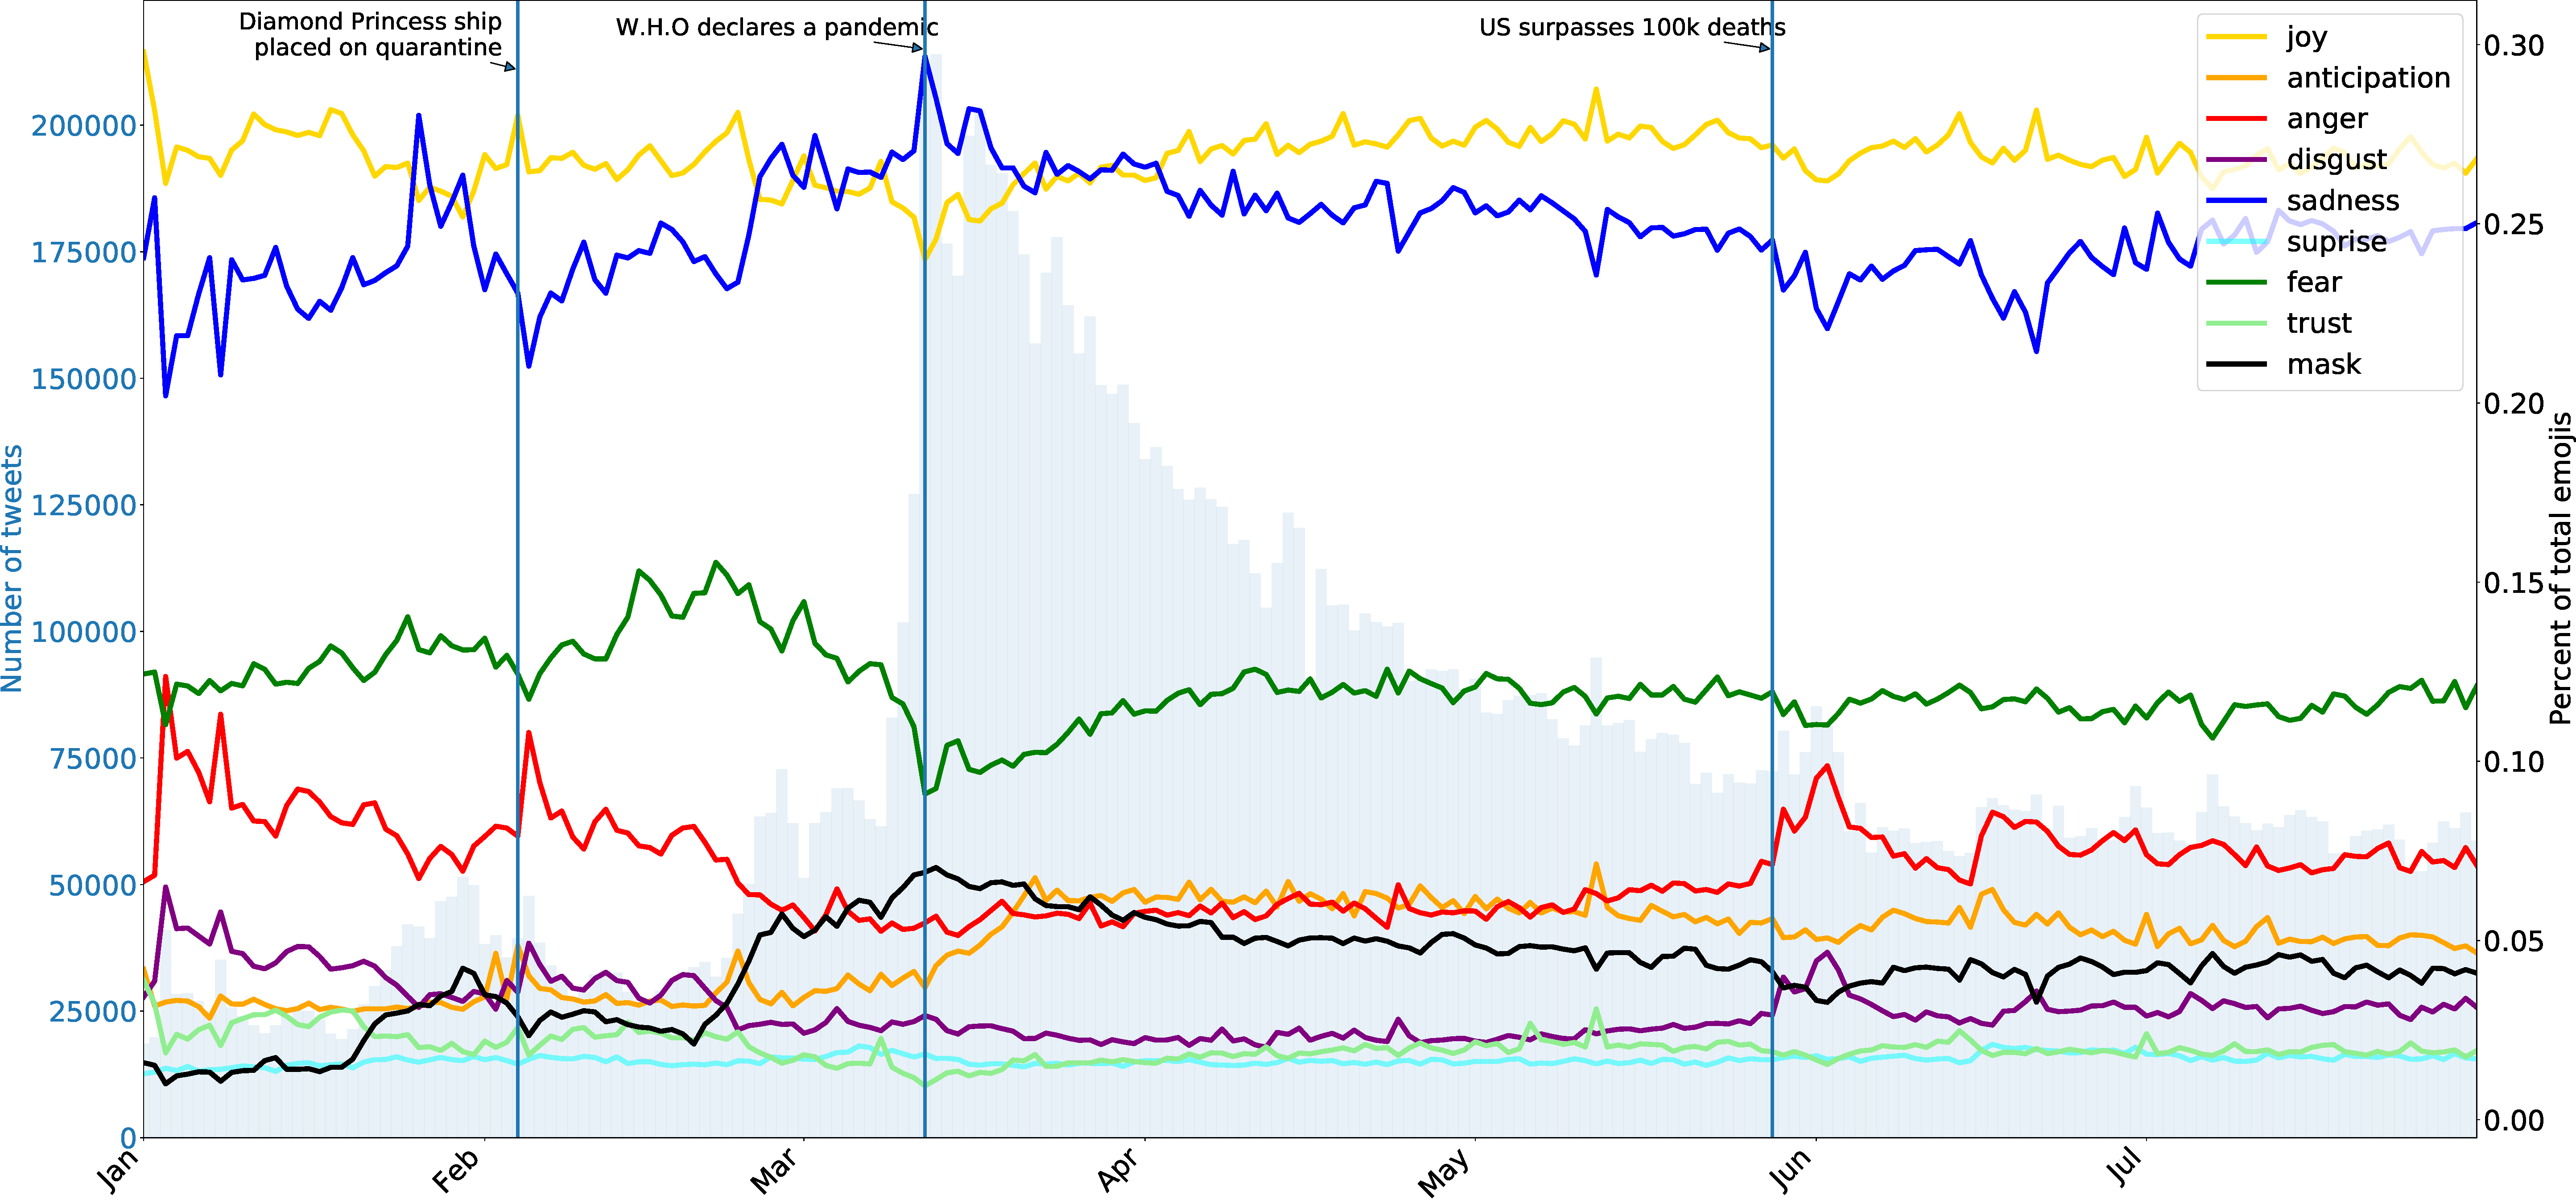
\includegraphics[width=\textwidth,height=2.5in]{images/twitter_graph_fix.pdf}
    \caption{
        The emotional content of tweets in the $\corona$ dataset changes over time and reacts to major news events.
        For example, when WHO declared a pandemic on $\XXX$, we can see that the amount of anticipation increases.
        \fixme{remove the whitespace on both sides of the plot}
        \fixme{the dates on the x-axis must have semantic meaning;
        the 1st of every month is a good choice}
        \fixme{the joy line is not readable; I realize that you're trying to make it match the plutchnik wheel, but you need to choose a darker color and probably make the line thicker.}
        \fixme{you should only be including date markers if there is something significant about the date that we can compare the prediction trends to.  For example, the ``WHO declares a pandemic'' is a good one because it corresponds to the dip in green, and ``10m cases is good because it has the rise in purple/red'', but ``WHO advises widespread mask use'' is not a good one because nothing happens in the graph.}
        \fixme{These arrows would be better done as vertical lines because we are pointing to a date, and not to a date and a number of tweets.}
        \fixme{the key background should be opaque, and the lines thicker so that we can see the colors easier}
        \fixme{are you currently including the Trump tweets in this plot?  It's a bit weird that the number of coronavirus tweets in Jan 1 is half the number in Aug 1, it should be like 0.1\%.  So I think you should remove the Trump tweets probably}
    }
        %The graph presents a bar plot of the number of tweets per day contained in the $\corona$ dataset;
    %a line plot for the 8 different emotions from the Plutchik wheel: joy, anticipation,anger, and for the use of the mask emoji.
    %We also include some of the important timelines of COVID-19:100 thousand,1 million,10 million cases alongside with some of the W.H.O responses
%}
    \label{fig:tweets_per_day_sent}
\end{figure}

\begin{figure}
    \centering
    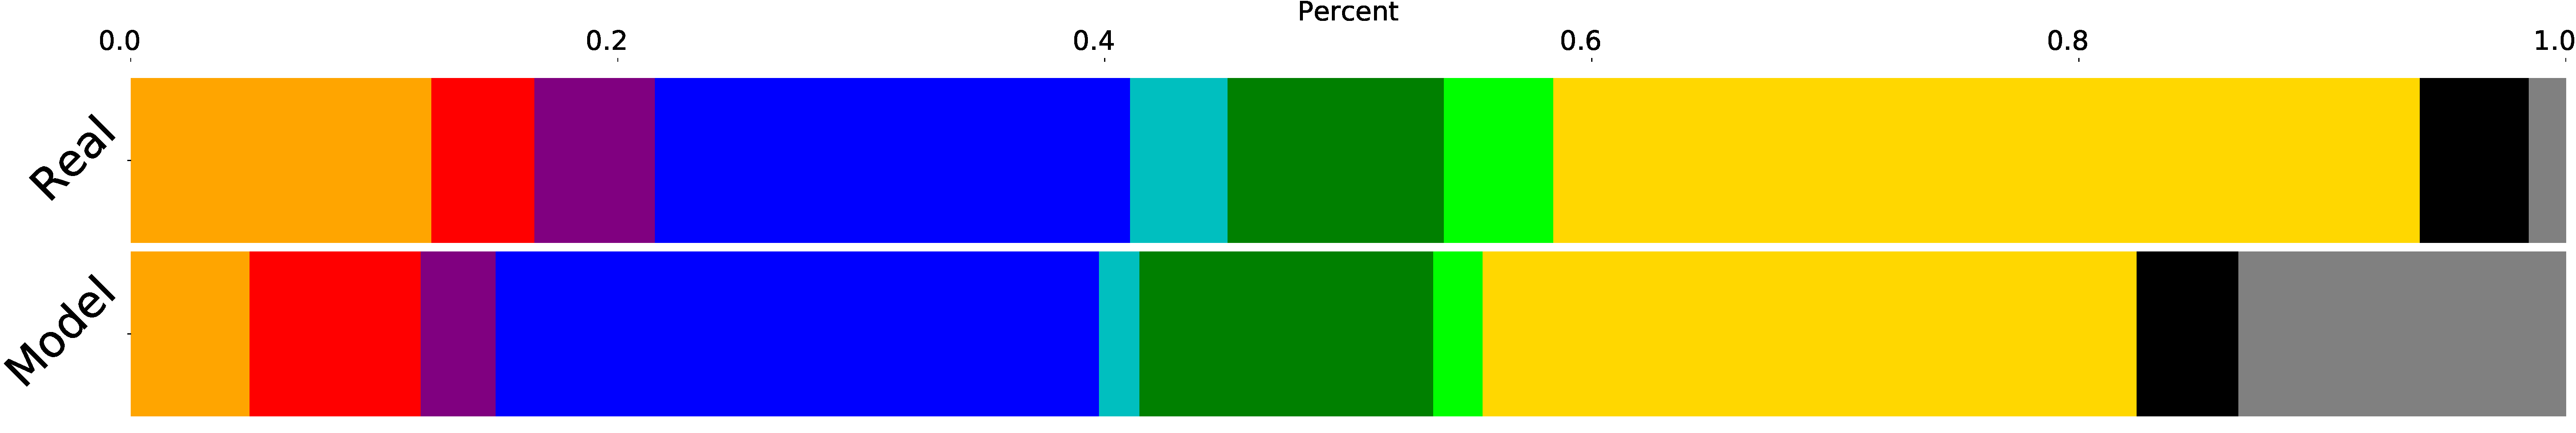
\includegraphics[width=\textwidth]{images/true_pred_fix.pdf}
    \caption{The true stacked bar presents the actual Plutchik wheel's mapped responses from the $\corona$ dataset while the predicted stacked bar graph presents the predicted emoji responses mapped to the Plutchik wheel following Figure  \ref{fig:Mapped_emojis} }
    \label{fig:actual vs pred}
\end{figure}

We are going to use one of the most common sentiment classification tools which is the Plutchik's wheel of emotions.
The classification \cite{} suggests 8 primary bipolar emotions: joy versus sadness; anger versus fear; trust versus disgust; 
and surprise versus anticipation as shown in Figure X. We then map the 80 emojis of the $\emoticon$ dataset
to those 8 emotions. Emojis which cannot be placed in those 8 categories are placed in the others category. 
Finally, we treated the mask-emoji as its own category due to the context of the $\corona$ dataset.
At this point, it is important to mention that emojis are used in different ways depending on people, cultures and context;
therefore, their use in social media is a product of polysemy. We attempt to map them according with: their core definitions and
our emoji use in social media. Table X shows the categories.  

Due to the fact that emojis such as crying-face with tears, dominate the $\emoticon$ dataset,
we allow the model to predict up to 5 unique emojis for one tweet, to promote more diversity among our results.
This way, the results can be more meaningful. Further research, can include a more balanced $\emoticon$ dataset.
We collect the 5 predicted emojis, and after mapping them to the correct sentiment category, we calculate their 
percent out of the total number of emojis predicted for that day. 
In order to understand the results we collected all the emojis from the tweets in the $\corona$ and mapped them to the categories in Figure \ref{fig:Mapped_emojis}.  

\section{Conclusion}

{ \color{blue} \lipsum[1-2] }

%%%%%%%%%%%%%%%%%%%%%%%%%%%%%%%%%%%%%%%%%%%%%%%%%%%%%%%%%%%%%%%%%%%%%%%%%%%%%%%%
%%%%%%%%%%%%%%%%%%%%%%%%%%%%%%%%%%%%%%%%%%%%%%%%%%%%%%%%%%%%%%%%%%%%%%%%%%%%%%%%
%%%%%%%%%%%%%%%%%%%%%%%%%%%%%%%%%%%%%%%%%%%%%%%%%%%%%%%%%%%%%%%%%%%%%%%%%%%%%%%%
%%%%%%%%%%%%%%%%%%%%%%%%%%%%%%%%%%%%%%%%%%%%%%%%%%%%%%%%%%%%%%%%%%%%%%%%%%%%%%%%
%%%%%%%%%%%%%%%%%%%%%%%%%%%%%%%%%%%%%%%%%%%%%%%%%%%%%%%%%%%%%%%%%%%%%%%%%%%%%%%%

\newpage
\fixme{The contents below will get put into the introduction.}
\section{Related Work}
\label{sec:related}
\subsection{Datasets:}
It is now worth mentioning previous datasets related with sentiment and emotion classification. The Sentiment Evaluation task 2018 \cite{mohammad-etal-2018-semeval} presents a dataset of English, Arabic and Spanish tweets extracted from Twitter API, labelled for an array of subtasks on inferring the affectual state of a person from their tweet. Seventy-five teams submitted to one or more of the five total tasks; however, most of the submissions where for the language English. 
\cite{liu2019dens} introduces the DENS dataset, for multi-class emotion analysis. By collecting both English classic literature and modern online narratives, and by fine-tuning the pre-trained uncased BERT-large model to the multi-class passage classification task they achieved a micro-F1 average score of 60.4\%.

\subsection{Pretrained models:}
On the domain of Pre-trained models for Natural Language Tasks, NVIDIA's researchers have published 
\cite{puri2018large} where by using Recurrent Neural Networks on a 40 GB Amazon Review dataset demonstrate 
the scalability and transfer of the RNNs. By utilizing mixed precision arithmetic and 
a 32k batch size distributed on 128 GPUs, they trained a character-level 4096-dimension mLSTM.
Furthermore, \cite{kant2018practical} claim that large-scale unsupervised language modeling combined 
with finetuning, provides a solution to the Multi-Emotion sentiment classification (Plutchik),
including those with label class imbalance and domain-specific context. By training an attention-based
transformer network on a Amazon 40 GB dataset, it outperforms the mLSTM model, while fine-tuning significantly 
improves performance for both Transformers and mLSTM.

\subsection{Examples of large scale sentiment analysis:}
\cite{mohammad2017stance} explores both stance and sentiment analysis by providing a dataset of annotated tweet-target pairs, organized
a shared Task competition on Stance. Their stance detection system achieved an F-score of 70.3 \%, where they utilized an linear-kernel
SVM classifier. Their stance dataset contains 4k tweets, aimed towards topics such as Hillary Clinton, Atheism and etc. In addition,
\cite{yang2015twitter} provides an insight into measuring emotional contagion in Social Media. By using SentiStrengh (a sentiment analysis program),
and the findings of a study which claims that individuals are more likely to adopt positive or negative emotions if these are over-expressed in
their social network; the authors pursuit in establishing a relation between the sentiment of a tweet and that of the tweets that its author may have seen in a short
time period preceding its posting. Interestingly, they raise ethical concerns as they require massive-scale content manipulation with unknown consequences for the individuals therein involved.
Finally, the provide noteworthy limitations of observational experiments.

\subsection{Emoji Prediction:}
It is now worth mentioning previous work on Emoji Prediction. \cite{barbieri-etal-2018-semeval} offered 2 subtasks for multilingual-emoji prediction: English and Spanish. By using Twitter API,
they located tweets either in the US (600k total) or in Spain (120k total). The tweets only included the one's with a single emoji and where limited to the top 20 emojis used across those countries. \cite{Tubingen_Olso} achieved 
the best performance in both the English and Spanish Tweets: F1-Score: 35.99 \%, F1-Score: 22.36 \% respectively obtained by an SVM classifier with bag-of-n-grams features. One of the best performing teams 
\cite{baziotis-etal-2018-ntua-slp}, achieved an F1-score of 35.36 \% on the English tweets, by using LSTM architecture with attention mechanism, initializing the embedding layer with word2vec and training end-to-end with back-propagation. 
The preprocessing tool they used was ekprahsis \cite{baziotis-etal-2017-datastories-semeval} which contains social tokenizer aimed for social media, spell correction and word segmentation which can be used for hashtag segmentation. Finally, \cite{towards_understanding_creatieve_lang}
explores both Irony Detection and the Emoji Prediction Task. They highlight that the knowledge the models gain is entirely from the corresponding training data, such training mechanism may work well for traditional text genres with formal sentences; however; 
it usually achieves an unsatisfiable performance with informal text, such as social media text.  By adopting a transfer learning model based on pretrained-BERT they achieved an F1-Score of 38.52 \% on the Emoji Prediction task. Issues raised by the authors were: overfitting 
due to the lack of more training data to fine-tune the system and time complexity.  
\section{Discussion}
\label{sec:discussion}


%\bibliographystyle{coling}
\bibliographystyle{plainnat}
\bibliography{main}

\end{document}
